\documentclass[a4paper,12pt]{article}

%% Language and font encodings
\usepackage[english, russian]{babel}
\usepackage[utf8x]{inputenc}
\usepackage{blindtext}
\usepackage[T1]{fontenc}
\usepackage[T2A]{fontenc}
\usepackage[a4paper,top=1.5 cm,bottom=2cm,left=3cm,right=3cm,marginparwidth=1.75cm]{geometry}
%% Useful packages
\usepackage{amsmath, amssymb}
\usepackage{wrapfig}
\usepackage{graphicx}
\usepackage[usenames]{color}
\usepackage[T1]{fontenc}
\usepackage{tikz}
\usetikzlibrary{arrows}
\usetikzlibrary{decorations.pathreplacing}
\usepackage[T2A]{fontenc}
\usepackage{color}
\usepackage{circuitikz} 
\graphicspath{{pic/}}
\definecolor{water} {rgb} {0.667, 0.855, 1}
\usepackage{pgfplots}
\usepackage{pgfplotstable}
\usetikzlibrary{circuits}
\usetikzlibrary{circuits.ee}
\usetikzlibrary{circuits.ee.IEC}
\usetikzlibrary{circuits.logic.IEC}
\usetikzlibrary{intersections}

\title{ДИФРАКЦИЯ СВЕТА НА ЗВУКОВОЙ ВОЛНЕ В ЖИДКОСТИ}
\date{Работа 4.3.2A}
\author{Ляликова Ирина, Б05-911}
\begin{document}
		\vspace{0.5 cm}
	\maketitle
	\vspace{0.5 cm}
	
	\textbf{Цель работы:} изучение дифракции света на синусоидальной акустической решетке и наблюдение фазовой решетки методом темного поля.
	
	\textbf{В работе используются:} оптическая скамья, осветитель, два длиннофокусных объектива, кювета с жидкостью, кварцевый излучатель с микрометрическим винтом, генератор звуковой частоты, линза, вертикальная нить на рейтере, микроскоп.
	
	\section*{Теоретическое введение}
	
	В работе используются оптическая скамья, осветитель, два длиннофокусных объектива, кювета с жидкостью, кварцевый излучатель с микрометрическим винтом, генератор звуковой частоты, линза, горизонтальная нить на рейтере, микроскоп. 
	
	При прохождении ультразвуковой волны через жидкость в ней возникают периодические неоднородности коэффициента преломления, создается фазовая решетка, которую мы считаем неподвижной ввиду малости скорости звука относительно скорости света. Показатель
	преломления n изменяется по закону:
	
	\begin{equation}\label{}
	n = n_0 (1 + m \cos \Omega x)
	\end{equation}
	
	Здесь $ \Omega = 2 \pi / \Lambda $ --- волновое число для ультразвуковой волны, $ m $ --- глубина модуляции $ n $ $ (m \ll 1 $).
	
	Положим фазу $ \phi $ колебаний световой волны на передней стенке кюветы равной нулю, тогда на задней поверхности она равна:
	
	\begin{equation}\label{}
	\phi  = k n L = \phi_0 (1 + m \cos \Omega x)
	\end{equation}
	
	Здесь $ L $ --- толщина жидкости в кювете, $ k = 2 \pi / \lambda $ --- волновое число для света.
	
	После прохождения через кювету световое поле есть совокупность плоских волн, распространяющихся под углами $ \theta $, соответствующими максимумам в дифракции Фраунгофера:
	
\begin{equation}\label{}	
	\Lambda \sin \theta_m = m \lambda
\end{equation}

	Этот эффект проиллюстрирован на рисунке 1.
	\begin{figure}[h!]
		\centering	
		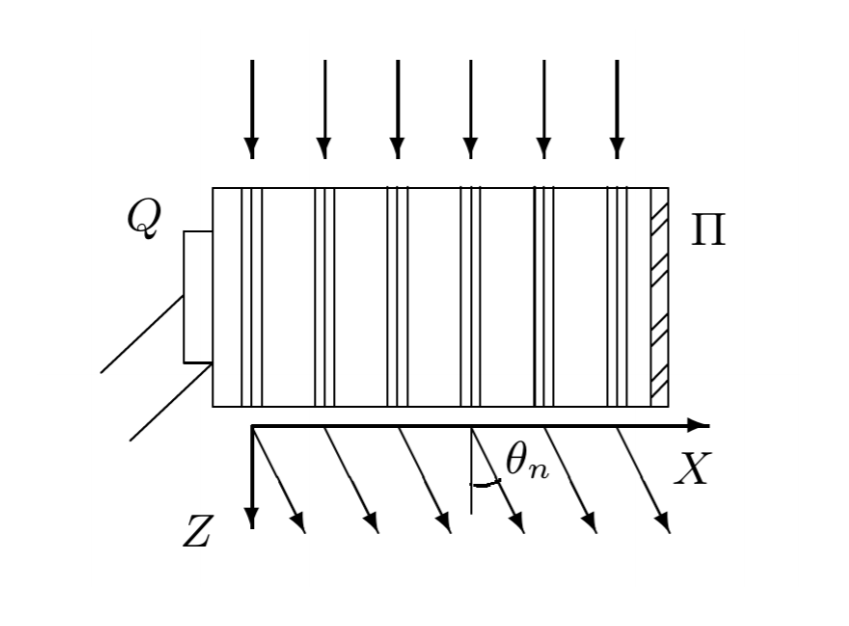
\includegraphics[width=0.3\textwidth]{wave.png}
		\caption{Дифракция световых волн на акустической решетке}
		\label{diff}
	\end{figure}
    Зная положение дифракционных максимумов, по формуле (1) легко определить длину ультразвуковой волны, учитывая малость $ \theta $: $ \sin \theta \approx \theta \approx l_m /F  $, где $ l_m $ --- расстояние от нулевого до последнего видимого максимума, $ F $ --- фокусное расстояние линзы. Тогда получим:
    	
    	\begin{equation}\label{}
    	 \Lambda = m \lambda F/ l_m 
    	\end{equation}
    	Скорость ультразвуковых волн в жидкости, где $ \nu $ --- частота колебаний излучателя:
    	
    \begin{equation}\label{}
    	v = \Lambda \nu 
    \end{equation}
    
    \textbf{Схема установки. }Схема установки приведена на рисунке 2. Источник света Л через светофильтр Ф и конденсор К освещает вертикальную щель $ S $, находящуюся в фокусе объектива $ O_1 $. После объектива параллельный световой пучок проходит через кювету С перпендикулярно акустической решетке, и дифракционная картина собирается в фокальной плоскости объектива $ O_2 $ , наблюдается при помощи микроскопа М.

    Предварительную настройку установки произведем в соответствии с инструкцией с зеленым фильтром, далее в работе используется красный.
    
    	\begin{figure}[h!]
    	\centering	
    	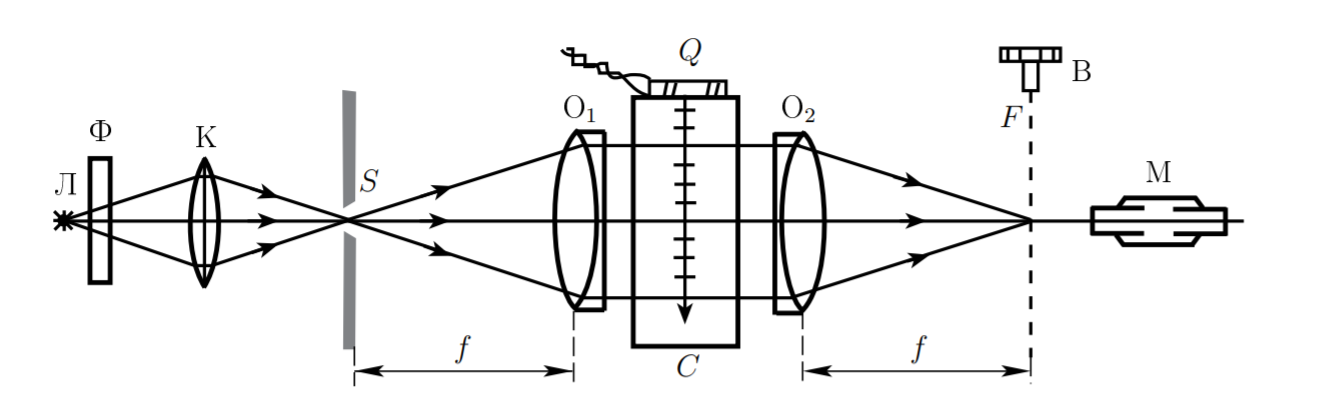
\includegraphics[width=0.7\textwidth]{stand.png}
    	\caption{Схема для наблюдения дифракции на акустической решетке}
    	\label{shema1}
    \end{figure}
    
    Параметры установки: фокусное расстояние объектива $F = 30 $ см, одно деление винта микроскопа составляет 20~мкм, полоса пропускания фильтра \mbox{$\lambda = 6400\pm 200$ Å}.
	
	\section*{Ход работы}
	\begin{enumerate}
	    \item Исследовали изменения дифракционной картины на красном свете. При увеличении частоты УЗ-генератора и приближении к 1,1~МГц проявляется дифракционная решетка: расстояние между максимумами растет.
	    
	    Измерили положения $ x_m $ дифракционных максимумов с помощью микроскопического винта для пяти частот. Для каждой полосы измерили крайние координаты и рассчитали среднее относительно нулевого максимума как координату полосы. Результаты измерений занесли в таблицах ниже. На основе каждой таблицы построили графики зависимости $ x_m (m) $.
	    
	    Для частоты $\nu_2=1{,}0116\pm 0{,}0001$ МГц:
	    \begin{center}
	    \begin{tabular}{|c|c|c|c|c|c|c|c|c|}
            \hline
            $m$ & -3 & -2 & -1 & 0 & 1 & 2 & 3 & 4 \\ \hline
            $l_m$, дел. & 2,15 & 2,40 & 2,70 & 3,00 & 3,35 & 3,60 & 3,90 & 4,20 \\ \hline
            $r_m$, дел. & 2,30 & 2,60 & 2,90 & 3,20 & 3,50 & 3,80 & 4,05 & 4,35 \\ \hline
            $x_m$, дел. & 2,225 & 2,50 & 2,80 & 3,10 & 3,425 & 3,70 & 3,975 & 4,275 \\ \hline
            $x_m$, мкм & -350 & -240 & -120 & 0 & 130 & 240 & 350 & 470 \\ \hline
        \end{tabular}
	    \end{center}
	\begin{figure}[!htb] \centering
		\begin{tikzpicture}
		\begin{axis}[
		width=15cm, height=8cm,
		xlabel={$m$}, ylabel={$x_m$, мкм},
		grid=major ]
		\addplot +[
		blue!20!black,
		mark = 0, only marks,
		] plot [
		error bars/.cd,
		x dir=both,	y dir=both,
		y fixed = 20, x fixed = 0,
		] table [
		x = x1, y = y1
		] {dat.dat};
		\addplot +[
		blue!20!black, mark = 0,
		] table [
		y={create col/linear regression={y=y1}}]
		{dat.dat};
		\end{axis}
		\end{tikzpicture}
		\caption{$x_m(m)$ на частоте $\nu_1$}
	\end{figure}
	
	\item Для частоты $\nu_1=1{,}2092\pm 0{,}0001$ МГц:
	    \begin{center}
	    \begin{tabular}{|c|c|c|c|c|c|c|c|}
            \hline
            $m$ & -3 & -2 & -1 & 0 & 1 & 2 & 3 \\ \hline
            $l_m$, дел. & 1,95 & 2,30 & 2,65 & 3,00 & 3,40 & 3,70 & 4,05 \\ \hline
            $r_m$, дел. & 2,15 & 2,50 & 2,85 & 3,20 & 3,55 & 3,85 & 4,20 \\ \hline
            $x_m$, дел. & 2,05 & 2,40 & 2,75 & 3,10 & 3,475 & 3,775 & 4,125 \\ \hline
            $x_m$, мкм & -420 & -280 & -140 & 0 & 150 & 240 & 410 \\ \hline
        \end{tabular}
	    \end{center}
	    
	\begin{figure}[!htb] \centering
		\begin{tikzpicture}
		\begin{axis}[
		width=15cm, height=8cm,
		xlabel={$m$}, ylabel={$x_m$, мкм},
		grid=major ]
		\addplot +[
		blue!20!black,
		mark = 0, only marks,
		] plot [
		error bars/.cd,
		x dir=both,	y dir=both,
		y fixed = 20, x fixed = 0,
		] table [
		x = x1, y = y2
		] {dat2.dat};
		\addplot +[
		blue!20!black, mark = 0,
		] table [
		y={create col/linear regression={y=y2}}]
		{dat2.dat};
		\end{axis}
		\end{tikzpicture}
		\caption{$x_m(m)$ на частоте $\nu_2$}
	\end{figure}
	
	\item Для частоты $\nu_3=2{,}9332\pm 0{,}0001$ МГц:
	    \begin{center}
	    \begin{tabular}{|c|c|c|c|c|c|c|c|}
            \hline
            $m$ & -2 & -1 & 0 & 1 & 2 & 3 \\ \hline
            $l_m$, дел. & 1,35 & 2,20 & 3,00 & 3,85 & 4,70 & 5,55 \\ \hline
            $r_m$, дел. & 1,60 & 2,40 & 3,20 & 4,0 & 4,90 & 5,70 \\ \hline
            $x_m$, дел. & 1,425 & 2,30 & 3,10 & 3,925 & 4,80 & 5,625 \\ \hline
            $x_m$, мкм & -670 & -320 & 0 & 330 & 680 & 1010 \\ \hline
        \end{tabular}
	    \end{center}
	\begin{figure}[!htb] \centering
		\begin{tikzpicture}
		\begin{axis}[
		width=15cm, height=8cm,
		xlabel={$m$}, ylabel={$x_m$, мкм},
		grid=major ]
		\addplot +[
		blue!20!black,
		mark = 0, only marks,
		] plot [
		error bars/.cd,
		x dir=both,	y dir=both,
		y fixed = 20, x fixed = 0,
		] table [
		x = x, y = y
		] {dat3.dat};
		\addplot +[
		blue!20!black, mark = 0,
		] table [
		y={create col/linear regression={y=y}}]
		{dat3.dat};
		\end{axis}
		\end{tikzpicture}
		\caption{$x_m(m)$ на частоте $\nu_3$}
	\end{figure}
	
	\item Дальше резонансы получать всё сложнее, к тому же в поле обзора попадает меньше полос либо полосы второго порядка не возникают. Графики по трём точкам строить бессмысленно. Для частоты $\nu_4=4{,}6086\pm 0{,}0001$~МГц:
	    \begin{center}
	    \begin{tabular}{|c|c|c|c|}
            \hline
            $m$ & -1 & 0 & 1 \\ \hline
            $l_m$, дел. & 1,70 & 3,00 & 4,35 \\ \hline
            $r_m$, дел. & 1,85 & 3,20 & 4,50 \\ \hline
            $x_m$, дел. & 1,775 & 3,10 & 4,425 \\ \hline
            $x_m$, мкм & -530 & 0 & 530 \\ \hline
        \end{tabular}
	    \end{center}
	\item Для частоты $\nu_5=5{,}1911\pm 0{,}0001$ МГц:
	    \begin{center}
	    \begin{tabular}{|c|c|c|c|}
            \hline
            $m$ & -1 & 0 & 1 \\ \hline
            $l_m$, дел. & 1,55 & 3,00 & 4,55 \\ \hline
            $r_m$, дел. & 1,70 & 3,20 & 4,65 \\ \hline
            $x_m$, дел. & 1,625 & 3,10 & 4,60 \\ \hline
            $x_m$, мкм & -590 & 0 & 600 \\ \hline
        \end{tabular}
	    \end{center}
	\end{enumerate}
	\section*{Обработка результатов}
	По составленным таблицам и коэффициентам наклона графика определим для каждой частоты $l_m/m$, чтобы по формуле (4) рассчитаем длины волн $\Lambda$ для всех частот.
	\begin{center}
	    \begin{tabular}{|c|c|c|c|c|c|}
	         \hline
	         $\nu$, МГц & 1,0116 & 1,2092 & 2,9332 & 4{,}6086 & 5{,}1911 \\ \hline
	         $l_m/m$, мкм & 117{,}8 & 136 & 335 & 530 & 595 \\ \hline
	         $\Delta(l_m/m)$, мкм &  0{,}9 & 3 & 5 & 20 & 20 \\ \hline
	         $\Lambda$, мкм & 1630 & 1410 & 573 & 362 & 323 \\ \hline
	         $\Delta\Lambda$, мкм & 50 & 60 & 30 & 13 & 10 \\ \hline
	    \end{tabular}
	\end{center}
	Построили график $\Lambda(1/\nu)$. По коэффициенту наклона определили скорость ультразвука в воде из формулы (5):
	$$v=1620\pm20\text{ м/с}.$$
	Для сравнения табличное значение составляет $v=1490$ м/с.
	\begin{figure}[!htb] \centering
		\begin{tikzpicture}
		\begin{axis}[
		width=15cm, height=8cm,
		ylabel={$\Lambda$, мкм}, xlabel={$1/\nu$, мкс},
		grid=major ]
		\addplot +[
		blue!20!black,
		mark = *, only marks, 
		] plot [
		error bars/.cd,
		x dir=both,	y dir=both,
		] table [
		x = x, y = y
		] {dat4.dat};
		\addplot +[
		blue!20!black, mark = 0,
		] table [
		y={create col/linear regression={y=y}}]
		{dat4.dat};
		\end{axis}
		\end{tikzpicture}
		\caption{$\Lambda(1/\nu)$}
	\end{figure}
    \section*{Вывод}
	Изучили явление дифракции света на ультразвуковой волне в воде. Сняли зависимость длины волны ультразвука от его частоты, и по этим параметрам получили значение скорости ультразвука в воде. Сравнили значение с табличным, точность экспериментального результата составила около 10\%.
\end{document}
